% !TEX root = CI_Adoption.tex

\section{Results and Discussion}

We sought to study how different software development practices change after CI adoption into the projects. 


\subsection{RQ1: Trends in Code Churn}

The first development practice we examine is code churn.
Our data consists of 567 projects, each with at least 500 nonmerge commits.

\noindent \underline{Exploratory Study} To explore general trends over time, we first look at code churn in months leading up to CI adoption.
Fig.~\ref{Fig:CodeChurnBefore} shows a boxplot of per-project median code churn for each of nine consecutive 30-day time intervals before CI adoption.
The vertical line in each boxplot is the median value of all per-project median, and the black dot is their average value.
We observe that for most part, the medians dance around 
10 and 12 lines of code churn per period, and the averages between 16 and 18 lines, with large variance and no obvious trend. The 30-day interval just before CI adoption seems to stand out and is higher than the rest.

Next, we look to the other side of the adoption point. Fig.~\ref{Fig:CodeChurnBefore} shows a boxplot of per-project median code churn for each of nine consecutive 30-day time intervals following CI adoption.
Here,  there seems to be a slight downward trend in both the medians and averages, the former drop monotonically from 13 down to 8 lines of code and the latter down to 15 lines of code.
However, we note the large variance around the medians.

The 30- and 60-day intervals just after the adoption point seem to be higher than the rest, and together with the 30-day interval just before adoption of CI seem to form a peak of increased code churn.
In conclusion, discounting the peak behavior in code churn around CI adoption time, we observe a small reduction in the amounts of code churn from before to after CI adoption.

% !TEX root = ../CI_Adoption.tex

\begin{table}[t] \centering
\small
  \caption{Model Coefficients for 566 Models of Code Churn}
  \label{Table:rddmodels}
\begin{tabular}{ l  r r r r }        
\hline 

 & $\beta$ & $\gamma$ & $\delta$ & $\beta + \delta$ \\ 
 \hline 
 \hline
not signif. & 504 & 508 & 514 & \\
\hline
signif., $>0$ & 45 & 28 & 10 & 13 \\
\hline
signif., $<0$ & 17 & 30 & 42 & 39 \\
\hline
\end{tabular}
\end{table}
\begin{figure}[!t]
\centering
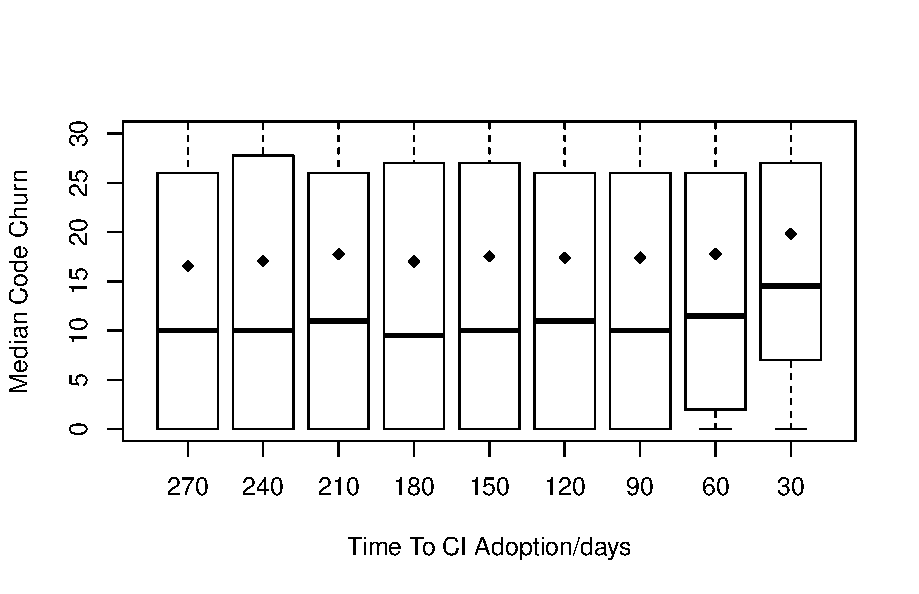
\includegraphics[width=0.5\textwidth]{churn_before.pdf}
\caption{The Code churn before CI adoption}
\label{Fig:CodeChurnBefore}
\end{figure}


\begin{figure}[!t]
\centering
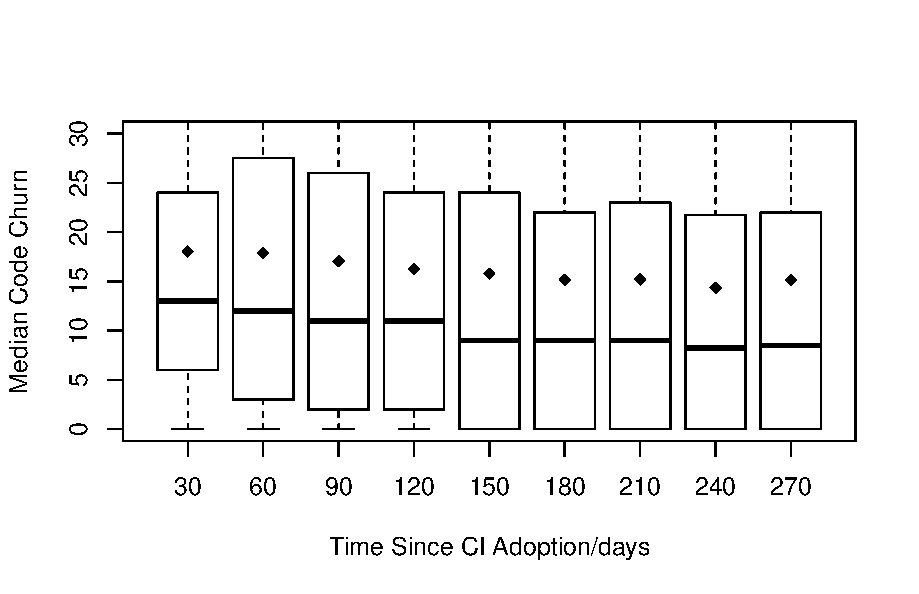
\includegraphics[width=0.5\textwidth]{churn_after.pdf}
\caption{The Code churn after CI adoption}
\label{Fig:CodeChurnAfter}
\end{figure}

\noindent \underline{Modeling Study} 
Guided by our observations from the exploratory study above, we proceed to quantify the trends we observed.
For each project, we fitted a sharp RDD model, as decribed before.
Because of the peak we observed, we eliminated the time point immediately before and the one immediately after the CI adoption time so as they do not throw off the regression models.
Table~\ref{Table:rddmodels} summarizes the results for the models on the remaining 16 time points.
Recall that $\beta$ is the slope before, $\gamma$ the size of the effect of CI introduction, $\delta$ is the divergence in the slopes before and after CI adoption, and $\beta + \delta$ the slope of the linear trend after CI adoption.

Of the 567 models, all but one could be fit to the data.
In 504 of the models, there was no significant linear relationship of code churn to time, i.e. there was no linear trend.
In 45 projects there was a rising trend before CI and in 17 projects a falling trend before CI.
Similarly, in 508 projects no effect of CI introduction on code churn was found. Among the 58 projects where an effect was significant, in about half (28) the trend was positive, i.e., code churn increased, and in the other half (30) it was negative, i.e., code churn decreased.
Interestingly, while in 514 projects no change of slope in the trends before and after CI adoption was found, in the 52 with significant change of trends a reduction in the slope was more prevalent than an increase by 4 to 1.
This carried over into trends following CI adoption: out of the 52 significant trend changes, 39 are downward trends, and only 13 are upward.

%Table XX: Projects with statistical negative trends after CI

\noindent \underline{Discussion}
Most of the projects could not be modeled with the RDD linear regression.
Some of the reasons for this are: dispersion of the data,
non-uniform distribution of the events across time, and project specific considerations that we could not model.

Our exploratory study showed a downward trend following CI adoption.
The modeling study showed that when linear trends were present, the downward ones after CI adoption were three times as frequent as the upward one, a reversal of the pattern in the trends before CI.
This is consistent with Fowler's good practices of CI, of committing more frequently and smaller pieces of code.
Still, most projects end up not following a trend after their adoption of CI, while still remaining active.

The increased code churn on both sides near the CI adoption time is arguably in line with expectations that more maintanance work may be going on in preparation for the transition to CI, and that the projects go through some adjustment/cleanup period right after.


\subsection{RQ2: Trends in Commit Frequency}

The second development practice we examine is commit frequency.
We use the same data as before, 567 projects, each with at least 500 nonmerge commits.

\begin{figure}[!t]
\centering
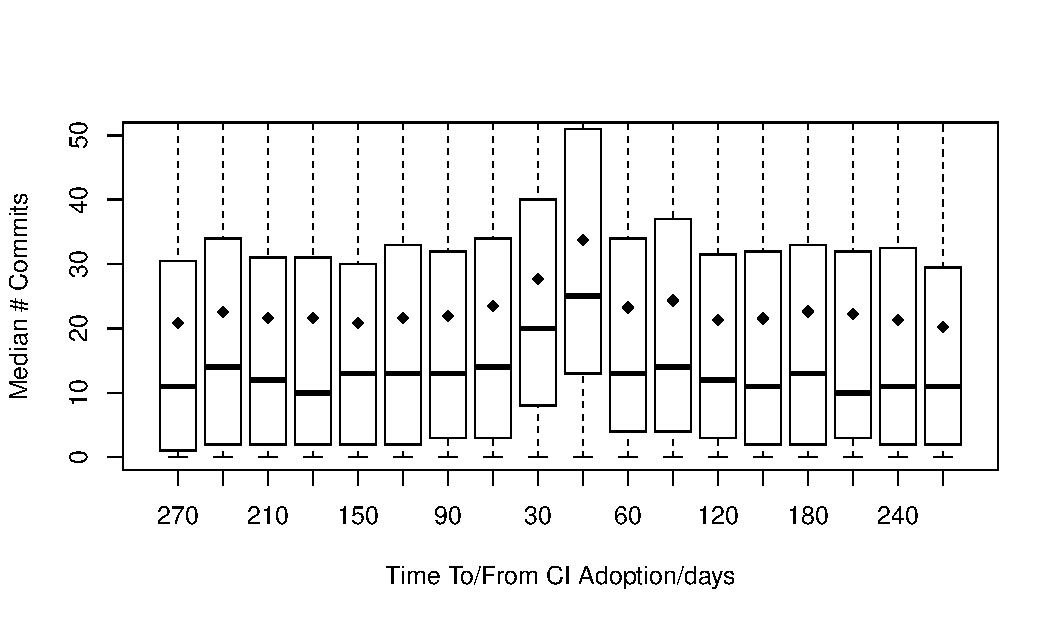
\includegraphics[width=0.5\textwidth]{numbercommits.pdf}
\caption{Commit frequency before and after CI adoption}
\label{Fig:NumberCommits}
\end{figure}

\noindent \underline{Exploratory Study} To explore general trends over time, we first look at commit frequency in the months leading up to CI adoption.
Figs.~\ref{Fig:NumberCommits} shows the boxplots of per-project median code churn for each of nine consecutive 30-day time intervals before CI adoption, and respectively, nine consecutive 30-day time intervals after CI adoption.
The vertical line in each boxplot is the median value of all per-project median, and the black dot is their average value.

As was the case with code churn, here we also see a peak in the 30-day interval just before and the one just after CI adoption.
Unlike for code churn, here we do not observe an apparent trend in the median or average commit frequency.

\noindent \underline{Modeling Study} 
As in RQ1, for each project, we fitted a sharp RDD model, as described before.
Table~\ref{Table:rddmodels_freq} summarizes the results.
We eliminated one time point on either side of the CI adoption time so as they do not throw off the regression models.
% !TEX root = ../CI_Adoption.tex

\begin{table}[t] \centering
\small
  \caption{Model Coefficients for 567 Models of Commit Frequency}
  \label{Table:rddmodels_freq}
\begin{tabular}{ l  r r r r }        
\hline 

 & $\beta$ & $\gamma$ & $\delta$ & $\beta + \delta$ \\ 
 \hline 
 \hline
not signif. & 452 & 466 & 454 & \\
\hline
signif., $\ge 0$ & 71 & 59 & 33 & 42 \\
\hline
signif., $<0$ & 44 & 42 & 80 & 71 \\
\hline
\end{tabular}
\end{table}

\begin{table}[t] \centering
\small
  \caption{Model Coefficients for 370 Models of Merge Commit Frequency}
  \label{Table:rddmodels_merge_freq}
\begin{tabular}{ l  r r r r }        
\hline 

 & $\beta$ & $\gamma$ & $\delta$ & $\beta + \delta$ \\ 
 \hline 
 \hline
not signif. & 296 & 307 & 301 & \\
\hline
signif., $\ge 0$ & 46 & 35 & 26 & 44 \\
\hline
signif., $<0$ & 28 & 28 & 43 & 30 \\
\hline
\end{tabular}
\end{table}

We were able to fit all 567 models to the data.
In 458 of the models, there was no significant linear relationship of commit frequency to time, i.e. there was no linear trend.
In 67 projects there was a rising trend in commit frequency before CI and in 42 projects a falling trend before CI.
Similarly, in 476 projects no effect of CI introduction on commit frequency was found. Among the 91 projects where an effect was significant, in about 50 the trend was positive, i.e., commit frequency increased, and in the rest it was negative, i.e., commit frequency decreased.
Interestingly, while in 468 projects no change of slope in the trends before and after CI adoption was found, in the 99 with significant change of trends a reduction in the slope was more prevalent than an increase by about 2 to 1.
This carried over into trends in commit frequency following CI adoption: out of the 99 significant trend changes, 66 are downward trends, and only 33 are upward.

\noindent \underline{Discussion}
As it is the case for the code churn, most of the projects could not be modeled with the RDD linear regression for 
the reasons similar to those in case of the code churn.

While our exploratory study did not suggest presence of a trend, the modeling study suggests that if a linear 
trend is present, then it is twice as likely to be decreasing as increasing. 
Given the expected increase in the frequency of commits expressed and encouraged by Fowler, this result might appear surprising.
One should keep in mind, however, that most projects do not show a trend.

\as{Vladimir, do you have a cross-combination data, such as \# decrease in churn AND increase in frequency?}



\subsection{RQ3: Trends in Issues}

\noindent \underline{Exploratory Study}
We follow the same approach as in RQ1 and RQ2 and compare the medians and the averages in the months
before and after the adoption of CI.
Fig.~\ref{Fig:IssuesBefore} and \ref{Fig:IssuesAfter} plot the number of issues per unit time period.
Observing these figures we can see that the months immediately 
preceding and following the adoption of CI exhibit the highest number of issues.
Following the adoption of CI the median of the number of issues seems to stabilize while averages do
not show a clear trend. 

\begin{figure}[!t]
\centering
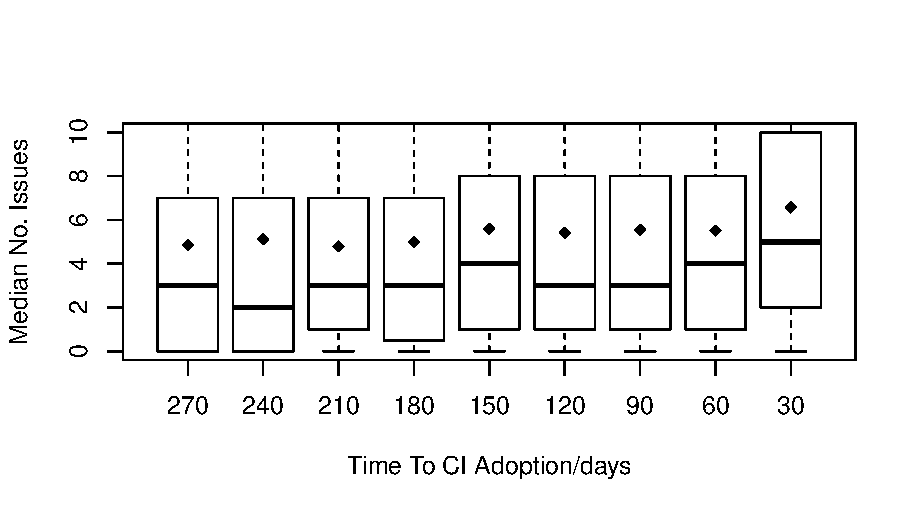
\includegraphics[width=0.5\textwidth]{issues_before.pdf}
\caption{Median number of issues before CI adoption}
\label{Fig:IssuesBefore}
\end{figure}


\begin{figure}[!t]
\centering
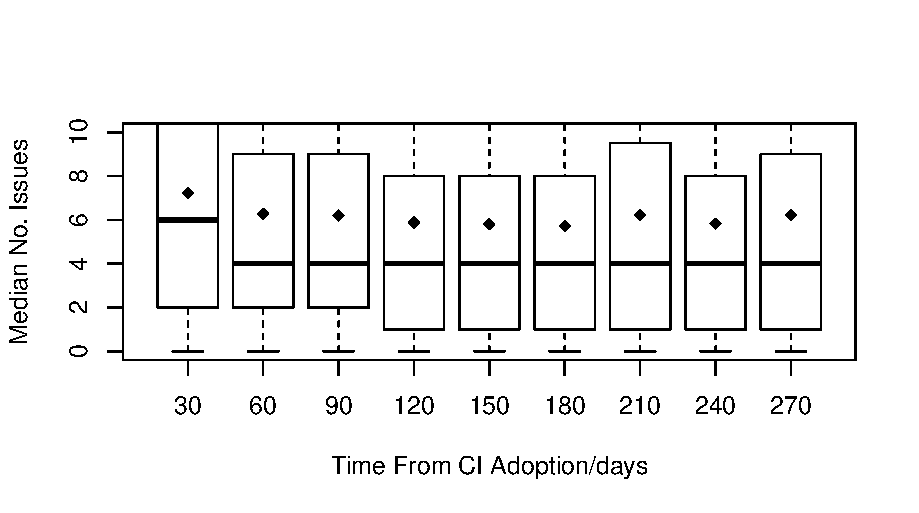
\includegraphics[width=0.5\textwidth]{issues_after.pdf}
\caption{Median number of issues after CI adoption}
\label{Fig:IssuesAfter}
\end{figure}

\noindent \underline{Modeling Study}
% !TEX root = ../CI_Adoption.tex

\begin{table}[t] \centering
\small
  \caption{Model Coefficients for 291 Models of Issues Frequency}
  \label{Table:rddmodels_freq}
\begin{tabular}{ l  r r r r }        
\hline 

 & $\beta$ & $\gamma$ & $\delta$ & $\beta + \delta$ \\ 
 \hline 
 \hline
not signif. & 230 & 254 & 242 & \\
\hline
signif., $>0$ & 43 & 26 & 14 & 15 \\
\hline
signif., $<0$ & 18 & 11 & 35 & 33 \\
\hline
\end{tabular}
\end{table}
Results of the RDD modeling are summarized in Table~\ref{Table:rddmodels_issues}.
Lower number of projects in Table~\ref{Table:rddmodels_issues} compared to Tables~\ref{Table:rddmodels} 
and~\ref{Table:rddmodels_freq} should not be surprising. 
Recall from Section~\ref{sec:dd} that to answer RQ3 we have focused on projects having at least 100 issues,
 reducing 567 projects used in RQ1 and RQ2 to 293.
We have fitted models to 291 projects of the 291, however in most cases we did not observe linear trends.
When a linear trend has been observed than it was more than twice more often decreasing than increasing.



\noindent \underline{Discussion}


The values of the $\gamma$'s for these models are right skewed, with average and median over 1. Thus, we conclude the effect of CI adoption led to an overall increase of one issue more per period.




\subsection{RQ4: Trends in Testing}

The second development practice we examine is testing and the evolution of the types of errors revealed by automated testing.
The data consists of XXX projects, each with at least YYY tests.

\noindent \underline{Exploratory Study} As before, we first look for general trends over time.
Fig.~\ref{Fig:Tests} shows a boxplot of per-project median number of tests per build, for each of five consecutive 60-day time intervals before CI adoption.
We aggregated the data here in 60 day intervals to make it easier to visualize the trend since the differences are small.
The vertical line in each boxplot is the median value of all per-project median, and the black dot is their average value.
We observe a monotonically increasing trend in both the medians, from 140 to 160 tests per build, and the means, from 205 to 245 tests per build, i.e. 15\% to 20\% increase. 

\begin{figure}[!t]
\centering
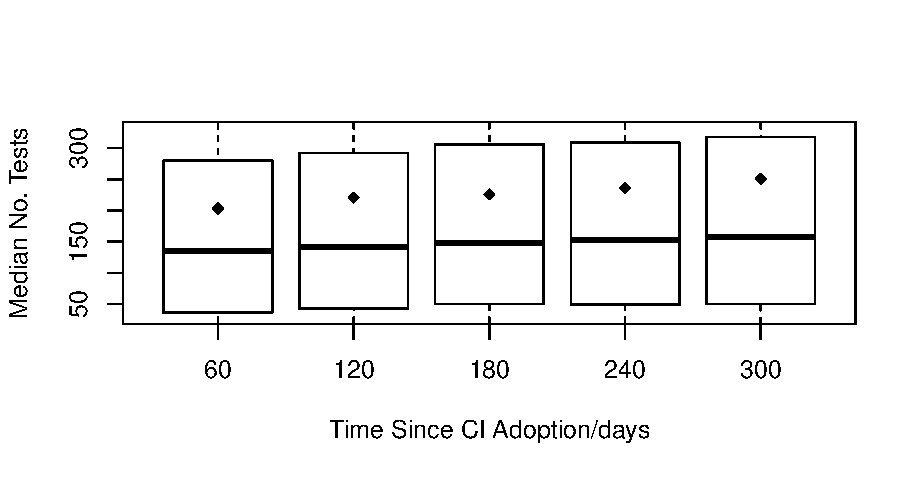
\includegraphics[width=0.5\textwidth]{tests.pdf}
\caption{Unit tests per build following CI adoption}
\label{Fig:Tests}
\end{figure}

\noindent \underline{Error Types Study}

\begin{figure}[!t]
\centering
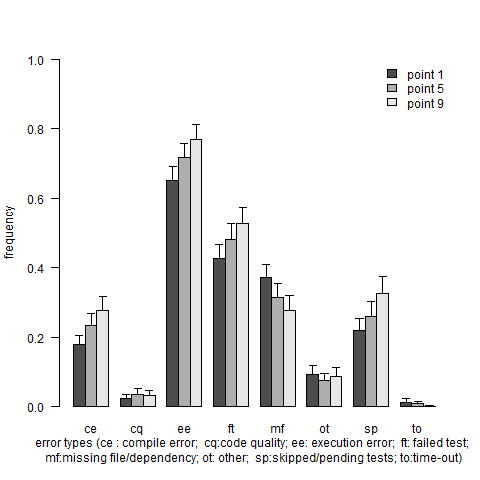
\includegraphics[width=0.5\textwidth]{plot_together.png}
\caption{Evolution of Error Types Since CI Adoption}
\label{Fig:BugTypes}
\end{figure}

\noindent \underline{Discussion}

